\documentclass[journal]{IEEEtran}

%\usepackage[retainorgcmds]{IEEEtrantools}
%\usepackage{bibentry}
\usepackage{xcolor,soul,framed} %,caption

\colorlet{shadecolor}{yellow}
% \usepackage{color,soul}
\usepackage[pdftex]{graphicx}
\graphicspath{{../pdf/}{../jpeg/}}
\DeclareGraphicsExtensions{.pdf,.jpeg,.png}

\usepackage[cmex10]{amsmath}
%Mathabx do not work on ScribTex => Removed
%\usepackage{mathabx}
\usepackage{array}
\usepackage{mdwmath}
\usepackage{mdwtab}
\usepackage{eqparbox}
\usepackage{url}


% ----------------------------------------------

% Definitions of languages: ------------
\usepackage{listings}
\lstdefinestyle{cStyle}{
  basicstyle=\scriptsize,
  breakatwhitespace=false,
  breaklines=true,
  captionpos=b,
  keepspaces=true,
  numbersep=5pt,
  showspaces=false,
  gobble=4,
  tabsize=4,
  showstringspaces=false,
  showtabs=false,
}
\renewcommand*{\lstlistingname}{Code}

% ----------------------------------------------




% \hyphenation{op-tical net-works semi-conduc-tor}

%\bstctlcite{IEEE:BSTcontrol}


%=== TITLE & AUTHORS ====================================================================
\begin{document}
\bstctlcite{IEEEexample:BSTcontrol}
    \title{Neural Networks}
  \author{Carlos~Matheus~Barros~da~Silva,~\IEEEmembership{Computer Engineering Bachelor Student of ITA}\\Prof. Marcos~Ricardo~Omena~de~Albuquerque~Máximo}

% The paper headers
\markboth{INSTITUTO TECNOLÓGICO DE AERONÁUTICA, May~2019
}{Neural Networks}

% ====================================================================
\maketitle



% === ABSTRACT ==============================================================
% ============================================================================
\begin{abstract}

This paper evaluates a shallow Neural Network by test it in diferent scenarios with two simple tests and a color segmentaion test.

It was observed that the Neural Network worked fine for those porposes, and in some case the result was really good, in the greater than function test case, for exemple.

For the color segmentation, the Neural Network also provided a concise well segmented result.

% === KEYWORDS ===============================================================
% ============================================================================
\begin{IEEEkeywords}
    Simple Evolution Strategy, SES, Covariance Matrix Adaptation Evolution Strategy, CMA-ES, optimization
\end{IEEEkeywords}
\end{abstract}

\IEEEpeerreviewmaketitle

% ====================================================================
% ====================================================================
% ====================================================================


% === I. INTRODUCTION ========================================================
% =============================================================================
\section{Introduction}

\IEEEPARstart{N}{e}ural networks (NN) are computing systems vaguely inspired by the biological neural networks and astrocytes that constitute animal brains. The neural network itself is not an algorithm, but rather a framework for many different machine learning algorithms to work together and process complex data inputs. Such systems "learn" to perform tasks by considering examples, generally without being programmed with any task-specific rules. For example, in image recognition, they might learn to identify images that contain cats by analyzing example images that have been manually labeled as "cat" or "no cat" and using the results to identify cats in other images. They do this without any prior knowledge about cats, for example, that they have fur, tails, whiskers and cat-like faces. Instead, they automatically generate identifying characteristics from the learning material that they process.

An NN is based on a collection of connected units or nodes called artificial neurons, which loosely model the neurons in a biological brain. Each connection, like the synapses in a biological brain, can transmit a signal from one artificial neuron to another. An artificial neuron that receives a signal can process it and then signal additional artificial neurons connected to it.

In common NN implementations, the signal at a connection between artificial neurons is a real number, and the output of each artificial neuron is computed by some non-linear function of the sum of its inputs. The connections between artificial neurons are called 'edges'. Artificial neurons and edges typically have a weight that adjusts as learning proceeds. The weight increases or decreases the strength of the signal at a connection. Artificial neurons may have a threshold such that the signal is only sent if the aggregate signal crosses that threshold. Typically, artificial neurons are aggregated into layers. Different layers may perform different kinds of transformations on their inputs. Signals travel from the first layer (the input layer), to the last layer (the output layer), possibly after traversing the layers multiple times.

The original goal of the NN approach was to solve problems in the same way that a human brain would. However, over time, attention moved to performing specific tasks, leading to deviations from biology. Artificial neural networks have been used on a variety of tasks, including computer vision, speech recognition, machine translation, social network filtering, playing board and video games and medical diagnosis.

% ==========================================================================
\section{Neural Network Implementation}

The implementation was based on the file \textit{neural network}. The essence of the implementation is on the methods \textit{forward propagation}, \textit{compute gradient back propagation} and \textit{back propagation}.

Those methods can be seen on the codes from Code \ref{code:forward} to Code \ref{code:compute}.

\lstinputlisting[
    language=python,
    caption={Code of \textit{forward propagation} method},
    label={code:forward},
    style=cStyle,
    firstline=35,
    lastline=59
]{./../code/neural_network.py}

\lstinputlisting[
    language=python,
    caption={Code of \textit{back propagation} method},
    label={code:back},
    style=cStyle,
    firstline=134,
    lastline=149
]{./../code/neural_network.py}

\lstinputlisting[
    language=python,
    caption={Code of \textit{compute gradient back propagation} method},
    label={code:compute},
    style=cStyle,
    firstline=86,
    lastline=132
]{./../code/neural_network.py}

\section{Neural Network Analysis}

In this analysis was used two test functions: \textit{sum greater than} and \textit{xor}.

The Neural Network performed very well on \textit{sum greater than} function. On the graphs represented by the images from Image \ref{img:greater_cost} to Image \ref{img:greater_cost}

\begin{figure}
  \begin{center}
  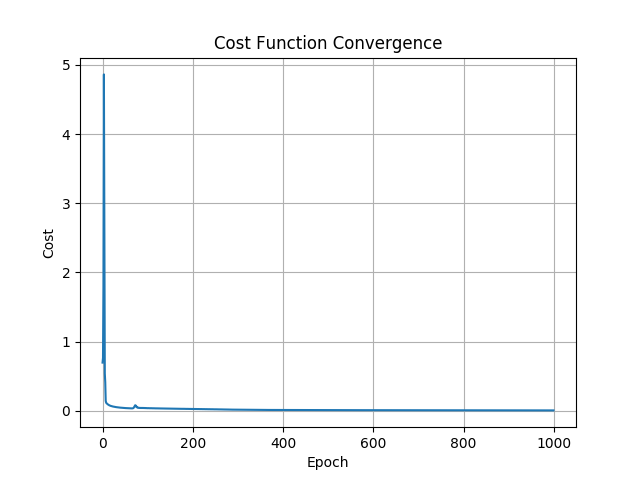
\includegraphics[width=2.8in]{./../code/result_greater_than/cost_function_convergence.png}
  \caption{Convergence of cost function on greater than function test case}
  \label{img:greater_cost}
  \end{center}
\end{figure}

\begin{figure}
  \begin{center}
  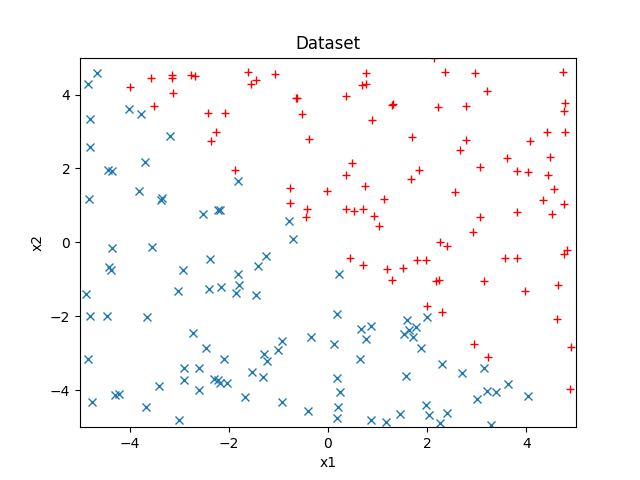
\includegraphics[width=2.8in]{./../code/result_greater_than/dataset.png}
  \caption{Dataset of greater than function}
  \label{img:greater_data_set}
  \end{center}
\end{figure}

\begin{figure}
  \begin{center}
  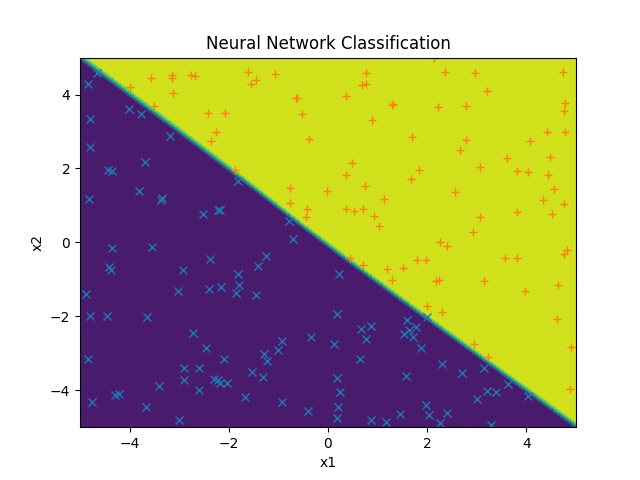
\includegraphics[width=2.8in]{./../code/result_greater_than/neural_net_classification.png}
  \caption{Neural Network Classification on greater than function}
  \label{img:greater_classification}
  \end{center}
\end{figure}

The Neural Network performed well on \textit{xor} function. On the graphs represented by the images from Image \ref{img:xor_cost} to Image \ref{img:xor_classification}. It is also possible to see that in this case it heapped some overfit causing some distorsion and leading to some mistakes on the data set on the graph represented by the Image \ref{img:xor_classification}.

\begin{figure}
  \begin{center}
  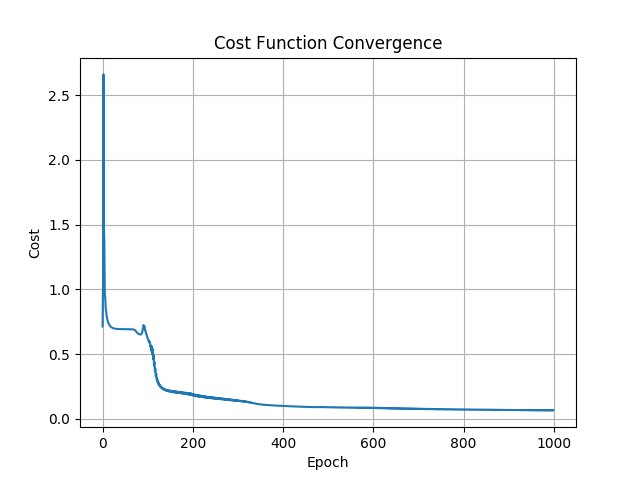
\includegraphics[width=2.8in]{./../code/result_xor/cost_function_convergence.png}
  \caption{Convergence of cost function on xor function test case}
  \label{img:xor_cost}
  \end{center}
\end{figure}

\begin{figure}
  \begin{center}
  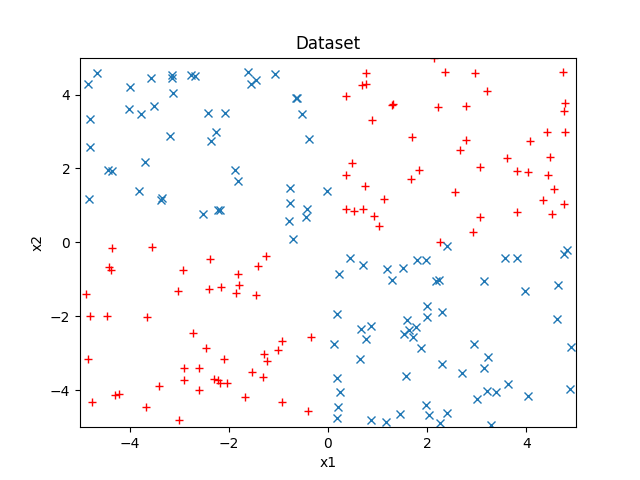
\includegraphics[width=2.8in]{./../code/result_xor/dataset.png}
  \caption{Dataset of xor function}
  \label{img:xor_data_set}
  \end{center}
\end{figure}

\begin{figure}
  \begin{center}
  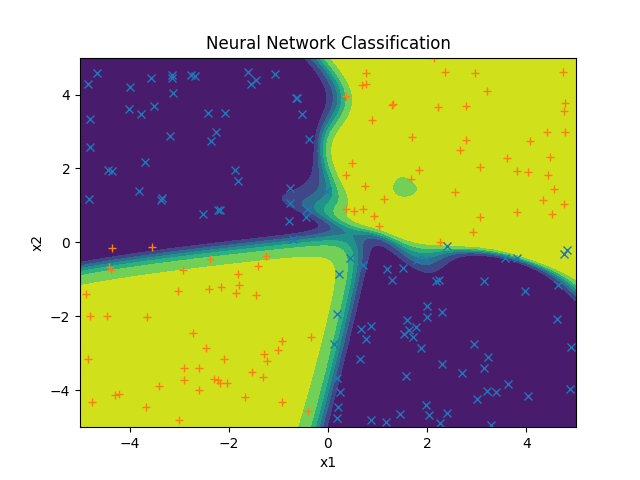
\includegraphics[width=2.8in]{./../code/result_xor/neural_net_classification.png}
  \caption{Neural Network Classification on xor function}
  \label{img:xor_classification}
  \end{center}
\end{figure}

\subsection{Neural Network Analysis on Color Segmentation}

In order to do a color segmentation, this Neural Network performed very well. This performance can be seen on the results figures on from Image \ref{img:result_original_img} to Image \ref{img:result_convergence}.

\begin{figure}
  \begin{center}
  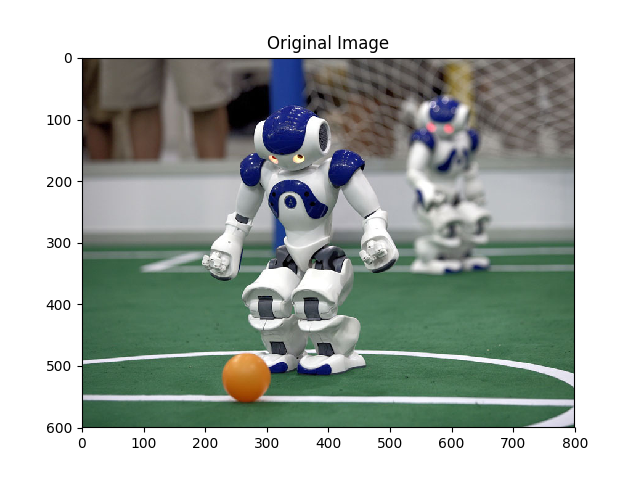
\includegraphics[width=2.8in]{./../code/result/original_image.png}
  \caption{Original image, before segmentation}
  \label{img:result_original_img}
  \end{center}
\end{figure}

\begin{figure}
  \begin{center}
  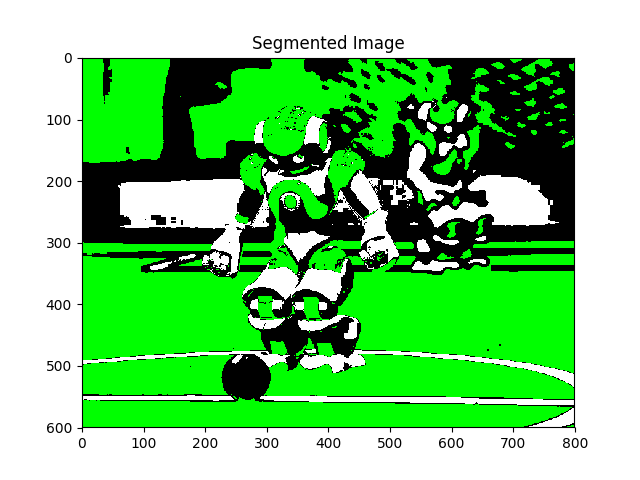
\includegraphics[width=2.8in]{./../code/result/segmented_image.png}
  \caption{Segmented image output}
  \label{img:result_segmented_img}
  \end{center}
\end{figure}

\begin{figure}
  \begin{center}
  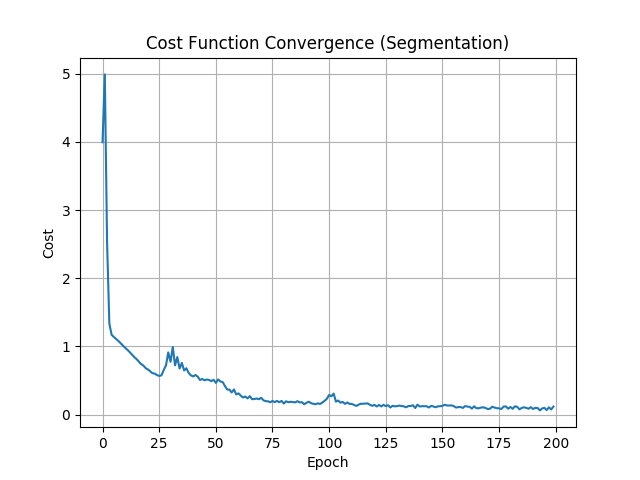
\includegraphics[width=2.8in]{./../code/result/cost_function_convergence_segmentation.png}
  \caption{Neural Network convergence of cost function on image color segmentation problem}
  \label{img:result_convergence}
  \end{center}
\end{figure}

\section {Conclusion}

It was clear, therefore, that the Neural Network worked as expected. Both test cases (greater than function and xor function) the Neural Network worked as expected.

For the color segmentation, the Neural Network also provided a concise well segmented result.

\vfill
\end{document}
